% 2009 年江西卷理科第 11 题：四个平面区域（阴影部分），周率依次为 τ1、τ2、τ3、τ4。
% 来源 PDF：gaokaomath-src/普通高考/2009/2009江西理.pdf
% SHA-256：64f70e9750ae2736476d825abdc20639c64a2dfe6c22493b64e710108d5c49e7
% 原页：2009江西理.pdf 第 1 页（A3 三栏）第 2 栏，书页码 533。
% 绘制依据：
%   图 1 为三级台阶形（外接正方形边长 3，周长 12，直径 3√2）；
%   图 2 为大圆内由两个半径减半的半圆拼成的太极形，左半外圆为虚线；
%   图 3 为两尖峰夹一谷的图形（底边 2.4、峰高 1.8、谷高 0.65）；
%   图 4 为正六角星（外接圆半径 1.2，内接六边形顶点半径 1.2/√3）。
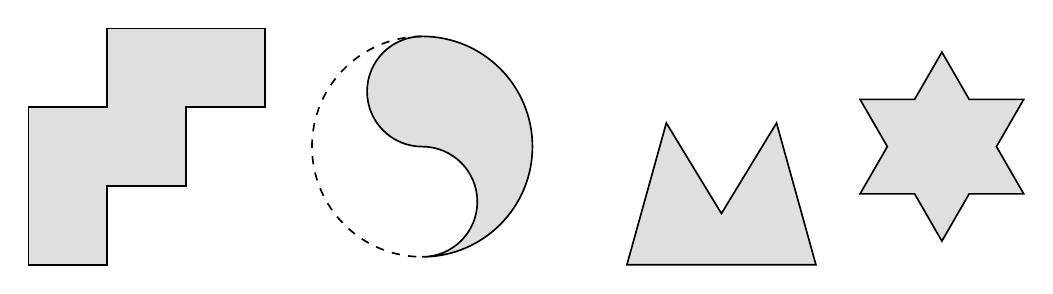
\begin{tikzpicture}[semithick, every node/.style={inner sep=1pt}]

  % ---------- 图 1：三级台阶形 ----------
  \begin{scope}[shift={(0,0)}]
    \fill[gray!25] (0,0) -- (1,0) -- (1,1) -- (2,1) -- (2,2) -- (3,2) -- (3,3)
      -- (1,3) -- (1,2) -- (0,2) -- cycle;
    \draw (0,0) -- (1,0) -- (1,1) -- (2,1) -- (2,2) -- (3,2) -- (3,3)
      -- (1,3) -- (1,2) -- (0,2) -- cycle;
  \end{scope}

  % ---------- 图 2：太极形 ----------
  \begin{scope}[shift={(5.0,1.5)}, scale=1.4]
    \fill[gray!25]
      (0,1) arc[start angle=90, end angle=-90, radius=1]
      arc[start angle=-90, end angle=90, radius=0.5]
      arc[start angle=-90, end angle=-270, radius=0.5]
      -- cycle;
    \draw[dashed] (0,1) arc[start angle=90, end angle=270, radius=1];
    \draw (0,1) arc[start angle=90, end angle=-90, radius=1]
      arc[start angle=-90, end angle=90, radius=0.5]
      arc[start angle=-90, end angle=-270, radius=0.5];
  \end{scope}

  % ---------- 图 3：双峰形 ----------
  \begin{scope}[shift={(7.6,0)}]
    \fill[gray!25] (0,0) -- (2.4,0) -- (1.9,1.8) -- (1.2,0.65) -- (0.5,1.8) -- cycle;
    \draw (0,0) -- (2.4,0) -- (1.9,1.8) -- (1.2,0.65) -- (0.5,1.8) -- cycle;
  \end{scope}

  % ---------- 图 4：正六角星 ----------
  \begin{scope}[shift={(11.6,1.5)}, scale=1.6]
    \fill[gray!25]
      (0,0.75) -- (0.2165,0.375) -- (0.6495,0.375) -- (0.433,0)
      -- (0.6495,-0.375) -- (0.2165,-0.375) -- (0,-0.75) -- (-0.2165,-0.375)
      -- (-0.6495,-0.375) -- (-0.433,0) -- (-0.6495,0.375) -- (-0.2165,0.375) -- cycle;
    \draw
      (0,0.75) -- (0.2165,0.375) -- (0.6495,0.375) -- (0.433,0)
      -- (0.6495,-0.375) -- (0.2165,-0.375) -- (0,-0.75) -- (-0.2165,-0.375)
      -- (-0.6495,-0.375) -- (-0.433,0) -- (-0.6495,0.375) -- (-0.2165,0.375) -- cycle;
  \end{scope}

\end{tikzpicture}
